\chapter{Array}
\section{LC 0001 - Two Sum}\label{lc0001}
Given an array of integers {\colorbox{CodeBackground}{\lstinline|nums|}} and an integer {\colorbox{CodeBackground}{\lstinline|target|}}, return indices of the two numbers such that they add up to target.\\

You may assume that each input would have \ul{exactly one solution}, and you may not use the same element twice.

\subsection*{Solution {\scriptsize\color{gray}\Coffeecup\hspace{1mm}Time $O(n)$, Space $O(n)$}}
\begin{lstlisting}
std::vector<int> twoSum(std::vector<int>& nums, int target) {
	std::unordered_map<int, int> val2comp_idx;
	for (int i = 0; i < nums.size(); ++i) {
		if (val2comp_idx.find(nums[i]) == val2comp_idx.end()) {
			val2comp_idx[target - nums[i]] = i;
		} else {
			return {i, val2comp_idx[nums[i]]};
		}
	}
	return {};
}
\end{lstlisting}

\subsection*{Related}
\begin{itemize}
\item \hyperref[lc0001]{LC 0001 - Two Sum}
\item \hyperref[lc0167]{LC 0167 - Two Sum II - Input Array Is Sorted}
\item \hyperref[lc0015]{LC 0015 - 3Sum}
\item \hyperref[lc0018]{LC 0018 - 4Sum}
\end{itemize}

\subsection*{Related - Hash Map For Searching Two Related Elements}
\begin{itemize}
\item \hyperref[lc0001]{LC 0001 - Two Sum}
\item \hyperref[lc0560]{LC 0560 - Subarray Sum Equals Target}
\item \hyperref[lc0523]{LC 0523 - Subarray Sum is Multiple of Target}
\item \hyperref[lc0525]{LC 0525 - Binary Subarray with Equal Zeros and Ones}
\end{itemize}

\section{LC 0167 - Two Sum II - Input Array Is Sorted}\label{lc0167}
Given a {\colorbox{CodeBackground}{\lstinline|1|}}-indexed array of integers {\colorbox{CodeBackground}{\lstinline|numbers|}} that is already sorted in \ul{non-decreasing order} ({\colorbox{CodeBackground}{\lstinline|nums.size() >= 2|}}), find two numbers such that they add up to a specific {\colorbox{CodeBackground}{\lstinline|target|}} number. Let these two numbers be {\colorbox{CodeBackground}{\lstinline|numbers[index1]|}} and {\colorbox{CodeBackground}{\lstinline|numbers[index2]|}} where {\colorbox{CodeBackground}{\lstinline|1 <= index1 < index2 <= numbers.size()|}}. \\

Return the indices of the two numbers, {\colorbox{CodeBackground}{\lstinline|index1|}} and {\colorbox{CodeBackground}{\lstinline|index2|}} as an integer array {\colorbox{CodeBackground}{\lstinline|[index1, index2]|}} of length {\colorbox{CodeBackground}{\lstinline|2|}}.\\

You may assume that there is \ul{exactly one solution}, and you may not use the same element twice.\\

Examples:
\begin{itemize}
	\item {\colorbox{CodeBackground}{\lstinline|numbers = [2,7,11,15], target = 9 --> [1,2]|}}
	\item {\colorbox{CodeBackground}{\lstinline|numbers = [2,3,4], target = 6 --> [1,3]|}}
	\item {\colorbox{CodeBackground}{\lstinline|numbers = [-1,0], target = -1 --> [1,2]|}}
\end{itemize}

\subsection*{Solution - Two Pointers {\scriptsize\color{gray}\Coffeecup\hspace{1mm}Time $O(n)$, Space $O(1)$}}
\begin{lstlisting}
std::vector<int> twoSum(std::vector<int>& numbers, int target) {
  int left = 0;
  int right = numbers.size() - 1;
  while (left < right) {
    int sum = numbers[left] + numbers[right];
    if (sum == target) {
      return {left + 1, right + 1};
    } else if (sum < target) {
      ++left;
    } else {
      --right;
    }
  }
  return {};
}
\end{lstlisting}

\subsection*{Related}
\begin{itemize}
\item \hyperref[lc0001]{LC 0001 - Two Sum}
\item \hyperref[lc0167]{LC 0167 - Two Sum II - Input Array Is Sorted}
\item \hyperref[lc0015]{LC 0015 - 3Sum}
\item \hyperref[lc0018]{LC 0018 - 4Sum}
\end{itemize}

\subsection*{Related - Two Pointers + Inward Search}
\begin{itemize}
\item \hyperref[lc0011]{LC 0011 - Container With Most Water}
\item \hyperref[lc0167]{LC 0167 - Two Sum II - Input Array Is Sorted}
\item \hyperref[lc0015]{LC 0015 - 3Sum}
\item \hyperref[lc0018]{LC 0018 - 4Sum}
\end{itemize}

\section{LC 0015 - 3Sum}\label{lc0015}
Given an integer array {\colorbox{CodeBackground}{\lstinline|nums|}} ({\colorbox{CodeBackground}{\lstinline|nums.size() >= 3|}}), return all the triplets {\colorbox{CodeBackground}{\lstinline|[nums[i], nums[j], nums[k]]|}} such that {\colorbox{CodeBackground}{\lstinline| i != j|}}, {\colorbox{CodeBackground}{\lstinline|i != k|}}, and {\colorbox{CodeBackground}{\lstinline|j != k|}}, and {\colorbox{CodeBackground}{\lstinline|nums[i] + nums[j] + nums[k] == 0|}}. \\

Note that the solution set must not contain duplicate triplets.\\

Examples:
\begin{itemize}
\item {\colorbox{CodeBackground}{\lstinline|nums = [-1,0,1,2,-1,-4] --> [[-1,-1,2],[-1,0,1]]|}}
\item {\colorbox{CodeBackground}{\lstinline|nums = [0,1,1] --> []|}}
\item {\colorbox{CodeBackground}{\lstinline|nums = [0,0,0] --> [[0,0,0]]|}}
\end{itemize}

\subsection*{Solution - Two Pointers {\scriptsize\color{gray}\Coffeecup\hspace{1mm}Time $O(n^2)$, Space $O(1)$}}
\begin{lstlisting}
std::vector<std::vector<int>> threeSum(std::vector<int>& nums) {
  std::vector<std::vector<int>> result;
  std::sort(nums.begin(), nums.end());
  for (int i = 0; i < nums.size(); ++i) {
    if (i > 0 && nums[i] == nums[i - 1]) { continue; }
    int target = -nums[i];
    int left = i + 1;
    int right = nums.size() - 1;
    while (left < right) {
      int sum = nums[left] + nums[right];
      if (sum == target) {
        result.push_back({nums[i], nums[left], nums[right]});
        while (left < right && nums[left] == nums[left + 1]) { ++left; }
        ++left;
        while (left < right && nums[right] == nums[right - 1]) { --right; }
        --right;
      } else if (sum < target) {
        ++left;
      } else {
        --right;
      }
    }
  }
  return result;
}
\end{lstlisting}

\subsection*{Related}
\begin{itemize}
\item \hyperref[lc0001]{LC 0001 - Two Sum}
\item \hyperref[lc0167]{LC 0167 - Two Sum II - Input Array Is Sorted}
\item \hyperref[lc0015]{LC 0015 - 3Sum}
\item \hyperref[lc0018]{LC 0018 - 4Sum}
\end{itemize}

\subsection*{Related - Two Pointers + Inward Search}
\begin{itemize}
\item \hyperref[lc0011]{LC 0011 - Container With Most Water}
\item \hyperref[lc0167]{LC 0167 - Two Sum II - Input Array Is Sorted}
\item \hyperref[lc0015]{LC 0015 - 3Sum}
\item \hyperref[lc0018]{LC 0018 - 4Sum}
\end{itemize}

\section{LC 0018 - 4Sum}\label{lc0018}
Given an array {\colorbox{CodeBackground}{\lstinline|nums|}} of {\colorbox{CodeBackground}{\lstinline|n|}} ({\colorbox{CodeBackground}{\lstinline|n >= 1|}}) integers, return an array of all the unique quadruplets {\colorbox{CodeBackground}{\lstinline|[nums[a], nums[b], nums[c], nums[d]]|}} such that:
\begin{itemize}
\item {\colorbox{CodeBackground}{\lstinline|0 <= a, b, c, d < n|}}
\item {\colorbox{CodeBackground}{\lstinline|a|}}, {\colorbox{CodeBackground}{\lstinline|b|}}, {\colorbox{CodeBackground}{\lstinline|c|}}, and {\colorbox{CodeBackground}{\lstinline|d|}} are distinct.
\item {\colorbox{CodeBackground}{\lstinline|nums[a] + nums[b] + nums[c] + nums[d] == target|}}
\end{itemize}

You may return the answer in any order.\\

Examples:
\begin{itemize}
\item {\colorbox{CodeBackground}{\lstinline|nums = [1,0,-1,0,-2,2], target = 0 --> [[-2,-1,1,2],[-2,0,0,2],[-1,0,0,1]]|}}
\item {\colorbox{CodeBackground}{\lstinline|nums = [2,2,2,2,2], target = 8 --> [[2,2,2,2]]|}}
\end{itemize}

\subsection*{Solution - Two Pointers {\scriptsize\color{gray}\Coffeecup\hspace{1mm}Time $O(n^3)$, Space $O(1)$}}
\begin{lstlisting}
std::vector<std::vector<int>> fourSum(std::vector<int>& nums, int target) {
  std::vector<std::vector<int>> result;
  std::sort(nums.begin(), nums.end());
  for (int i = 0; i < nums.size(); ++i) {
    for (int j = i + 1; j < nums.size(); ++j) {
      long two_sum_target = static_cast<long>(target) - nums[i] - nums[j];
      int left = j + 1;
      int right = nums.size() - 1;
      while (left < right) {
        long two_sum = nums[left] + nums[right];
        if (two_sum < two_sum_target) {
          left++;
        } else if (two_sum > two_sum_target) {
          right--;
        } else {
          std::vector<int> quadruplet(4, 0);
          quadruplet[0] = nums[i];
          quadruplet[1] = nums[j];
          quadruplet[2] = nums[left];
          quadruplet[3] = nums[right];
          result.push_back(quadruplet);
          while (left < right && nums[left] == quadruplet[2]) { ++left; }
          while (left < right && nums[right] == quadruplet[3]) { --right; }
        }
      }
      while (j + 1 < nums.size() && nums[j + 1] == nums[j]) { ++j; }
    }
    while (i + 1 < nums.size() && nums[i + 1] == nums[i]) { ++i; }
  }
  return result;
}
\end{lstlisting}

\subsection*{Related}
\begin{itemize}
\item \hyperref[lc0001]{LC 0001 - Two Sum}
\item \hyperref[lc0167]{LC 0167 - Two Sum II - Input Array Is Sorted}
\item \hyperref[lc0015]{LC 0015 - 3Sum}
\item \hyperref[lc0018]{LC 0018 - 4Sum}
\end{itemize}

\subsection*{Related - Two Pointers + Inward Search}
\begin{itemize}
\item \hyperref[lc0011]{LC 0011 - Container With Most Water}
\item \hyperref[lc0167]{LC 0167 - Two Sum II - Input Array Is Sorted}
\item \hyperref[lc0015]{LC 0015 - 3Sum}
\item \hyperref[lc0018]{LC 0018 - 4Sum}
\end{itemize}

\section{LC 0027 - Remove Element}\label{lc0027}
Given an integer array {\colorbox{CodeBackground}{\lstinline|nums|}} and an integer {\colorbox{CodeBackground}{\lstinline|val|}}, remove all occurrences of {\colorbox{CodeBackground}{\lstinline|val|}} in {\colorbox{CodeBackground}{\lstinline|nums|}} \ul{in-place}. The order of the elements may be changed. Then return the number of elements in {\colorbox{CodeBackground}{\lstinline|nums|}} which are not equal to {\colorbox{CodeBackground}{\lstinline|val|}}.\\

Consider the number of elements in {\colorbox{CodeBackground}{\lstinline|nums|}} which are not equal to {\colorbox{CodeBackground}{\lstinline|val|}} be {\colorbox{CodeBackground}{\lstinline|k|}}, to get accepted, you need to do the following things:
\begin{itemize}
	\item Change the array {\colorbox{CodeBackground}{\lstinline|nums|}} such that the first {\colorbox{CodeBackground}{\lstinline|k|}} elements of {\colorbox{CodeBackground}{\lstinline|nums|}} contain the elements which are not equal to {\colorbox{CodeBackground}{\lstinline|val|}}. The remaining elements of nums are not important as well as the size of {\colorbox{CodeBackground}{\lstinline|nums|}}.
	\item Return {\colorbox{CodeBackground}{\lstinline|k|}}.
\end{itemize}

Examples:
\begin{itemize}
	\item {\colorbox{CodeBackground}{\lstinline|nums = [3,2,2,3], val = 3 --> 2, nums = [2,2,_,_]|}}
	\item {\colorbox{CodeBackground}{\lstinline|nums = [0,1,2,2,3,0,4,2], val = 2 --> 5, nums = [0,1,4,0,3,_,_,_]|}}
\end{itemize}

\subsection*{Solution 1 - {\colorbox{CodeBackground}{\lstinline|std::remove()|}}}
\begin{lstlisting}
int removeElement(std::vector<int>& nums, int val) {
	return std::remove(nums.begin(), nums.end(), val) - nums.begin();
}
\end{lstlisting}

\subsection*{Solution 2}
\begin{lstlisting}
int removeElement(std::vector<int>& nums, int val) {
  int i = 0;  // pass-the-end idx of the reserved part
  for (int j = 0; j < nums.size(); ++j) {
    if (nums[j] != val) { nums[i++] = nums[j]; }
  }
  return i;
}
\end{lstlisting}

\section{LC 0026 - Remove Duplicates from Sorted Array}\label{lc0026}
Given an integer array {\colorbox{CodeBackground}{\lstinline|nums|}} sorted in \ul{non-decreasing order}, remove the duplicates \ul{in-place }such that each unique element appears only \ul{once}. The relative order of the elements should be kept the same. Then return the number of unique elements in {\colorbox{CodeBackground}{\lstinline|nums|}}.\\

Consider the number of unique elements of {\colorbox{CodeBackground}{\lstinline|nums|}} to be {\colorbox{CodeBackground}{\lstinline|k|}}, to get accepted, you need to do the following things:
\begin{itemize}
	\item Change the array {\colorbox{CodeBackground}{\lstinline|nums|}} such that the first {\colorbox{CodeBackground}{\lstinline|k|}} elements of {\colorbox{CodeBackground}{\lstinline|nums|}} contain the unique elements in the order they were present in {\colorbox{CodeBackground}{\lstinline|nums|}} initially. The remaining elements of {\colorbox{CodeBackground}{\lstinline|nums|}} are not important as well as the size of {\colorbox{CodeBackground}{\lstinline|nums|}}.
	\item Return {\colorbox{CodeBackground}{\lstinline|k|}}.
\end{itemize}

Examples:
\begin{itemize}
	\item {\colorbox{CodeBackground}{\lstinline|nums = [1,1,2] --> 2, nums = [1,2,_]|}}
	\item {\colorbox{CodeBackground}{\lstinline|nums = [0,0,1,1,1,2,2,3,3,4] --> 5, nums = [0,1,2,3,4,_,_,_,_,_]|}}
\end{itemize}

\subsection*{Solution 1 - {\colorbox{CodeBackground}{\lstinline|std::unique()|}}}
\begin{lstlisting}
int removeDuplicates(std::vector<int>& nums) {
	return std::unique(nums.begin(), nums.end()) - nums.begin();
}
\end{lstlisting}

\subsection*{Solution 2}
\begin{lstlisting}
int removeDuplicates(std::vector<int>& nums) {
  if (nums.size() <= 1) { return nums.size(); }
  int i = 1;  // past-the-end idx of reserved part
  for (int j = 1; j < nums.size(); ++j) {
    if (nums[j] != nums[i - 1]) { nums[i++] = nums[j]; }
  }
  return i;
}

\end{lstlisting}

\subsection*{Related}
\begin{itemize}
	\item \hyperref[lc0026]{LC 0026 - Remove Duplicates from Sorted Array}
	\item \hyperref[lc0080]{LC 0080 - Remove Duplicates from Sorted Array II}
	\item \hyperref[lc0083]{LC 0083 - Remove Duplicates from Sorted List}
	\item \hyperref[lc0082]{LC 0082 - Remove Duplicates from Sorted List II}
\end{itemize}

\section{LC 0080 - Remove Duplicates from Sorted Array II}\label{lc0080}
Given an integer array {\colorbox{CodeBackground}{\lstinline|nums|}} sorted in \ul{non-decreasing order}, remove some duplicates \ul{in-place} such that each unique element appears at most \ul{twice}. The relative order of the elements should be kept the same.\\

You must have the result be placed in the first part of the array {\colorbox{CodeBackground}{\lstinline|nums|}}. More formally, if there are {\colorbox{CodeBackground}{\lstinline|k|}} elements after removing the duplicates, then the first {\colorbox{CodeBackground}{\lstinline|k|}} elements of {\colorbox{CodeBackground}{\lstinline|nums|}} should hold the final result. It does not matter what you leave beyond the first {\colorbox{CodeBackground}{\lstinline|k|}} elements.\\

Return {\colorbox{CodeBackground}{\lstinline|k|}} after placing the final result in the first {\colorbox{CodeBackground}{\lstinline|k|}} slots of {\colorbox{CodeBackground}{\lstinline|nums|}}.\\

Examples:
\begin{itemize}
	\item {\colorbox{CodeBackground}{\lstinline|nums = [1,1,1,2,2,3] --> 5, nums = [1,1,2,2,3,_]|}}
	\item {\colorbox{CodeBackground}{\lstinline|nums = [0,0,1,1,1,1,2,3,3] --> 7, nums = [0,0,1,1,2,3,3,_,_]|}}
\end{itemize}

\subsection*{Solution}
\begin{lstlisting}
int removeDuplicates(std::vector<int>& nums) {
  if (nums.size() <= 2) { return nums.size(); }
  int i = 2;  // past-the-end idx of reserved part
  for (int j = 2; j < nums.size(); ++j) {
    if (nums[j] != nums[i - 2]) { nums[i++] = nums[j]; }
  }
  return i;
}
\end{lstlisting}

\subsection*{Related}
\begin{itemize}
	\item \hyperref[lc0026]{LC 0026 - Remove Duplicates from Sorted Array}
	\item \hyperref[lc0080]{LC 0080 - Remove Duplicates from Sorted Array II}
	\item \hyperref[lc0083]{LC 0083 - Remove Duplicates from Sorted List}
	\item \hyperref[lc0082]{LC 0082 - Remove Duplicates from Sorted List II}
\end{itemize}

\section{LC 0217 - Contains Duplicate}\label{lc0217}
Given a \ul{non-empty} integer array {\colorbox{CodeBackground}{\lstinline|nums|}}, return {\colorbox{CodeBackground}{\lstinline|true|}} if any value appears at least twice in the array, and return {\colorbox{CodeBackground}{\lstinline|false|}} if every element is distinct.\\

Examples:
\begin{itemize}
\item {\colorbox{CodeBackground}{\lstinline|nums = [1,2,3,1] --> true|}}
\item {\colorbox{CodeBackground}{\lstinline|nums = [1,2,3,4] --> false|}}
\item {\colorbox{CodeBackground}{\lstinline|nums = [1,1,1,3,3,4,3,2,4,2] --> true|}}
\end{itemize}

\subsection*{Solution 1 - Hash Set}
\begin{lstlisting}
bool containsDuplicate(std::vector<int>& nums) {
  std::unordered_set<int> seen;
  for (int num : nums) {
    if (!seen.insert(num).second) { return true; }
  }
  return false;
}
\end{lstlisting}

\subsection*{Solution 2 - Sorting}
\begin{lstlisting}
bool containsDuplicate(std::vector<int>& nums) {
  std::sort(nums.begin(), nums.end());
  for (int i = 0; i < nums.size() - 1; ++i) {
    if (nums[i] == nums[i + 1]) { return true; }
  }
  return false;
}
\end{lstlisting}

\subsection*{Related}
\begin{itemize}
\item \hyperref[lc0217]{LC 0217 - Contains Duplicate}
\item \hyperref[lc0219]{LC 0219 - Contains Duplicate II}
\end{itemize}

\section{LC 0219 - Contains Duplicate II}\label{lc0219}
{\hyperref[sec:sliding_window]{[Sliding Window]}}

\begin{tcolorbox}
\begin{itemize}
\item Check for duplicates in a sliding window across arrays/strings/lists.
\end{itemize}
\end{tcolorbox}

Given a \ul{non-empty} integer array {\colorbox{CodeBackground}{\lstinline|nums|}} and an integer {\colorbox{CodeBackground}{\lstinline|k|}} ({\colorbox{CodeBackground}{\lstinline|k >= 0|}}), return {\colorbox{CodeBackground}{\lstinline|true|}} if there are two distinct indices {\colorbox{CodeBackground}{\lstinline|i|}} and {\colorbox{CodeBackground}{\lstinline|j|}} in the array such that {\colorbox{CodeBackground}{\lstinline|nums[i] == nums[j]|}} and {\colorbox{CodeBackground}{\lstinline|std::abs(i - j) <= k|}}. \\

Examples:
\begin{itemize}
	\item {\colorbox{CodeBackground}{\lstinline|nums = [1,2,3,1], k = 3 --> true|}}
	\item {\colorbox{CodeBackground}{\lstinline|nums = [1,0,1,1], k = 1 --> true|}}
	\item {\colorbox{CodeBackground}{\lstinline|nums = [1,2,3,1,2,3], k = 2 --> false|}}
\end{itemize}

\subsection*{Solution 1 - Sliding Window + Hash Set {\scriptsize\color{gray}\Coffeecup\hspace{1mm}Time $O(n)$, Space $O(n)$}}
\begin{lstlisting}
bool containsNearbyDuplicate(std::vector<int>& nums, int k) {
  std::unordered_set<int> seen;
  for (int i = 0; i < nums.size(); ++i) {
    if (i > k) { seen.erase(nums[i - (k + 1)]); }
    if (!seen.insert(nums[i]).second) { return true; }
  }
  return false;
}
\end{lstlisting}

\subsection*{Solution 2 - Sliding Window + Hash Map {\scriptsize\color{gray}\Coffeecup\hspace{1mm}Time $O(n)$, Space $O(n)$}}
\begin{lstlisting}
bool containsNearbyDuplicate(std::vector<int>& nums, int k) {
  std::unordered_map<int, int> num2last_idx;
  for (int i = 0; i < nums.size(); ++i) {
    if (num2last_idx.find(nums[i]) != num2last_idx.end()
        && std::abs(i - num2last_idx[nums[i]]) <= k) {
      return true;
    }
    num2last_idx[nums[i]] = i;
  }
  return false;
}
\end{lstlisting}

\subsection*{Related}
\begin{itemize}
\item \hyperref[lc0217]{LC 0217 - Contains Duplicate}
\item \hyperref[lc0219]{LC 0219 - Contains Duplicate II}
\end{itemize}

\section{LC 0189 - Rotate Array}\label{lc0189}
Given an integer array {\colorbox{CodeBackground}{\lstinline|nums|}}, \ul{rotate the array to the right by {\colorbox{CodeBackground}{\lstinline|k|}} ({\colorbox{CodeBackground}{\lstinline|k >=0|}}) steps}.\\

Examples:
\begin{itemize}
	\item {\colorbox{CodeBackground}{\lstinline|nums = [1,2,3,4,5,6,7], k = 3 --> [5,6,7,1,2,3,4]|}}
	\item {\colorbox{CodeBackground}{\lstinline|nums = [-1,-100,3,99], k = 2 --> [3,99,-1,-100]|}}
\end{itemize}

\subsection*{Solution  {\scriptsize\color{gray}\Coffeecup\hspace{1mm}Time $O(n)$, Space $O(1)$}}
\begin{lstlisting}
void rotate(std::vector<int>& nums, int k) {
	k %= nums.size();
	// reverse the whole array
	std::reverse(nums.begin(), nums.end());
	// reverse the first k elements
	std::reverse(nums.begin(), nums.begin() + k);
	// reverse the rest of the array
	std::reverse(nums.begin() + k, nums.end());
}
\end{lstlisting}

\subsection*{Related}
\begin{itemize}
	\item \hyperref[lc0189]{LC 0189 - Rotate Array}
	\item \hyperref[lc0061]{LC 0061 - Rotate List}
\end{itemize}

\section{LC 0088 - Merge Sorted Array}\label{lc0088}
You are given two integer arrays {\colorbox{CodeBackground}{\lstinline|nums1|}} and {\colorbox{CodeBackground}{\lstinline|nums2|}}, sorted in \ul{non-decreasing order}, and two integers {\colorbox{CodeBackground}{\lstinline|m|}} and {\colorbox{CodeBackground}{\lstinline|n|}}, representing the number of elements in {\colorbox{CodeBackground}{\lstinline|nums1|}} and {\colorbox{CodeBackground}{\lstinline|nums2|}} respectively. Merge {\colorbox{CodeBackground}{\lstinline|nums1|}} and {\colorbox{CodeBackground}{\lstinline|nums2|}} into a single array sorted in \ul{non-decreasing order}.\\

The final sorted array should not be returned by the function, but instead be stored inside the array {\colorbox{CodeBackground}{\lstinline|nums1|}}. To accommodate this, {\colorbox{CodeBackground}{\lstinline|nums1|}} has a length of {\colorbox{CodeBackground}{\lstinline|m + n|}}, where the first {\colorbox{CodeBackground}{\lstinline|m|}} elements denote the elements that should be merged, and the last {\colorbox{CodeBackground}{\lstinline|n|}} elements are set to {\colorbox{CodeBackground}{\lstinline|0|}} and should be ignored. {\colorbox{CodeBackground}{\lstinline|nums2|}} has a length of {\colorbox{CodeBackground}{\lstinline|n|}}.\\

Example:
\begin{lstlisting}
	nums1 = [1,2,3,0,0,0], m = 3, nums2 = [2,5,6], n = 3 --> [1,2,2,3,5,6]
\end{lstlisting}

\subsection*{Solution {\scriptsize\color{gray}\Coffeecup\hspace{1mm}Time $O(m + n)$, Space $O(1)$}}
\begin{lstlisting}
void merge(std::vector<int>& nums1, int m, std::vector<int>& nums2, int n) {
	int i = m - 1;
	int j = n - 1;
	int k = m + n - 1;
	while (i >= 0 && j >= 0) {
		if (nums1[i] > nums2[j]) {
			nums1[k--] = nums1[i--];
		} else {
			nums1[k--] = nums2[j--];
		}
	}
	while (j >= 0) { nums1[k--] = nums2[j--]; }
}
\end{lstlisting}

\subsection*{Related - Merge Sort}
\begin{itemize}
	\item \hyperref[lc0088]{LC 0088 - Merge Sorted Array}
	\item \hyperref[lc0021]{LC 0021 - Merge Two Sorted Lists}
\end{itemize}

\section{LC 0252 - Meeting Rooms}\label{lc0252}
\hyperref[sec:interval_range]{[Interval \& Range]}\\

Given an array of meeting time {\colorbox{CodeBackground}{\lstinline|intervals|}} where {\colorbox{CodeBackground}{\lstinline|intervals[i] = [start_i, end_i]|}}, determine if a person could attend all meetings. (Hint: If no meetings overlap, the person can attend all meetings.) \\

Examples:
\begin{itemize}
\item {\colorbox{CodeBackground}{\lstinline|intervals = [[0,30],[5,10],[15,20]] --> false|}}
\item {\colorbox{CodeBackground}{\lstinline|intervals = [[7,10],[2,4]] --> true|}}
\end{itemize}

\subsection*{Solution - Sort By Start}
\begin{lstlisting}
bool canAttendMeetings(std::vector<std::vector<int>>& intervals) {
  std::sort(intervals.begin(), intervals.end(),
            [](const std::vector<int>& lhs, const std::vector<int>& rhs) {
              return lhs[0] < rhs[0];
            });
  for (int i = 1; i < intervals.size(); ++i) {
    if (intervals[i][0] < intervals[i - 1][1]) { return false; }
  }
  return true;
}
\end{lstlisting}

\subsection*{Related}
\begin{itemize}
\item \hyperref[lc0252]{LC 0252 - Meeting Rooms}
\item \hyperref[lc0253]{LC 0253 - Meeting Rooms II}
\end{itemize}

\section{LC 0057 - Insert Interval}\label{lc0057}
\hyperref[sec:interval_range]{[Interval \& Range]}\\

You are given an array of non-overlapping intervals {\colorbox{CodeBackground}{\lstinline|intervals|}} where {\colorbox{CodeBackground}{\lstinline|intervals[i] = [start_i, end_i]|}} represent the start and the end of the {\colorbox{CodeBackground}{\lstinline|i|}}th interval and {\colorbox{CodeBackground}{\lstinline|intervals|}} is sorted in ascending order by {\colorbox{CodeBackground}{\lstinline|start_i|}}. \\

You are also given an interval {\colorbox{CodeBackground}{\lstinline|newInterval = [start, end]|}} that represents the start and end of another interval.\\

Insert {\colorbox{CodeBackground}{\lstinline|newInterval|}} into {\colorbox{CodeBackground}{\lstinline|intervals|}} such that {\colorbox{CodeBackground}{\lstinline|intervals|}} is still sorted in ascending order by {\colorbox{CodeBackground}{\lstinline|start_i|}} and {\colorbox{CodeBackground}{\lstinline|intervals|}} still does not have any overlapping intervals (merge overlapping intervals if necessary).\\

Return {\colorbox{CodeBackground}{\lstinline|intervals|}} after the insertion.\\

Examples:
\begin{itemize}
\item {\colorbox{CodeBackground}{\lstinline|intervals = [[1,3],[6,9]], newInterval = [2,5] --> [[1,5],[6,9]]|}}
\item {\colorbox{CodeBackground}{\lstinline|intervals = [[1,2],[3,5],[6,7],[8,10],[12,16]], newInterval = [4,8] --> [[1,2],[3,10],[12,16]]|}}
\end{itemize}

\subsection*{Solution}
\begin{lstlisting}
std::vector<std::vector<int>> insert(std::vector<std::vector<int>>& intervals,
                                     std::vector<int>& new_interval) {
  std::vector<std::vector<int>> adjusted_intervals;
  int i = 0;
  // 1. intervals before new_interval
  while (i < intervals.size() && intervals[i][1] < new_interval[0]) {
    adjusted_intervals.push_back(intervals[i]);
    ++i;
  }
  // 2. intervals overlapping with new_interval
  while (i < intervals.size() && intervals[i][0] <= new_interval[1]) {
    new_interval[0] = std::min(new_interval[0], intervals[i][0]);
    new_interval[1] = std::max(new_interval[1], intervals[i][1]);
    ++i;
  }
  adjusted_intervals.push_back(new_interval);
  // 3. intervals after new_interval
  while (i < intervals.size()) {
    adjusted_intervals.push_back(intervals[i]);
    ++i;
  }
  return adjusted_intervals;
}
\end{lstlisting}

\section{LC 0986 - Intersections of Interval Lists}\label{lc0986}
\hyperref[sec:interval_range]{[Interval \& Range]}\\

You are given two lists of closed intervals, {\colorbox{CodeBackground}{\lstinline|interval_list1|}} and {\colorbox{CodeBackground}{\lstinline|interval_list2|}} (at least one of them is non-empty), where {\colorbox{CodeBackground}{\lstinline|interval_list1[i] = [start_i, end_i]|}} and {\colorbox{CodeBackground}{\lstinline|interval_list2[j] = [start_j, end_j]|}}.\\

Each list of intervals is \ul{pairwise disjoint} and \ul{in sorted order}.\\

Return the intersection of these two interval lists.\\

\begin{itemize}
\item Example 1:
\begin{lstlisting}
interval_list1 = [[0,2],[5,10],[13,23],[24,25]]
interval_list2 = [[1,5],[8,12],[15,24],[25,26]]
--> [[1,2],[5,5],[8,10],[15,23],[24,24],[25,25]]
\end{lstlisting}
\begin{figure}[H]
\centering
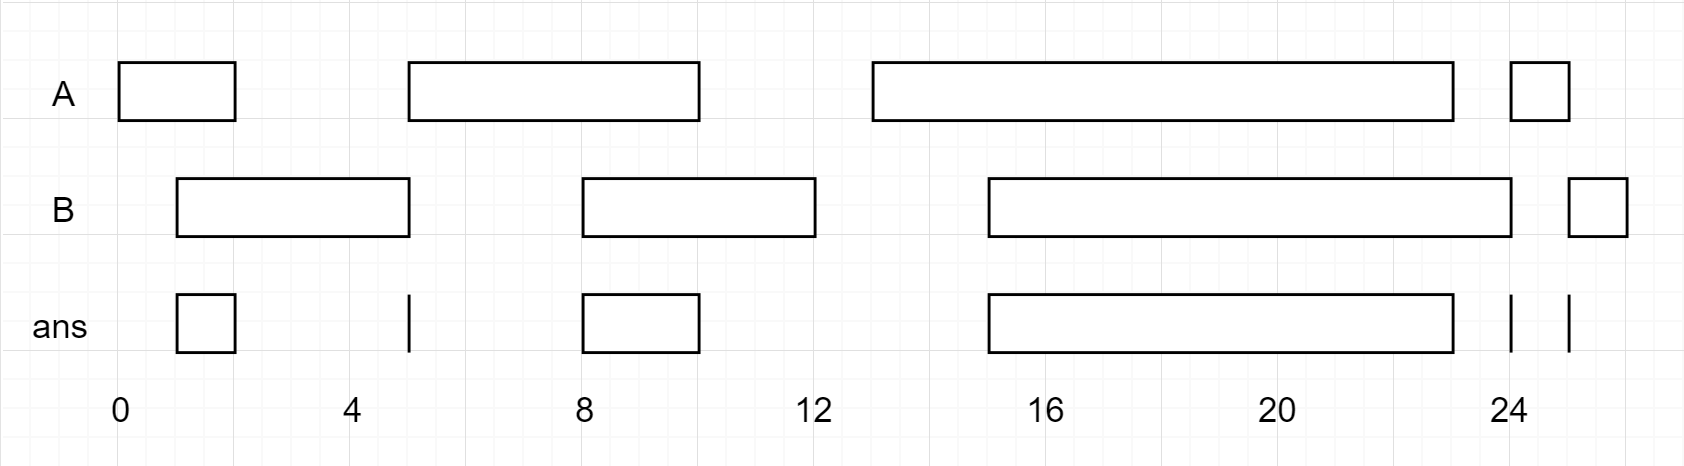
\includegraphics[width=0.7\linewidth]{images/lc0986_eg1}
\end{figure}
\item Example 2:
\begin{lstlisting}
interval_list1 = [[1,3],[5,9]]
interval_list2 = []
--> []
\end{lstlisting}
\end{itemize}

\subsection*{Solution}
\begin{lstlisting}
std::vector<std::vector<int>> intervalIntersection(
    std::vector<std::vector<int>>& interval_list1,
    std::vector<std::vector<int>>& interval_list2) {
  std::vector<std::vector<int>> intersections;
  int i = 0;
  int j = 0;
  while (i < interval_list1.size() && j < interval_list2.size()) {
    // check if there is an intersection
    int start_max = std::max(interval_list1[i][0], interval_list2[j][0]);
    int end_min = std::min(interval_list1[i][1], interval_list2[j][1]);
    if (start_max <= end_min) { intersections.push_back({start_max, end_min}); }
    // move the pointer with the smaller end
    if (interval_list1[i][1] < interval_list2[j][1]) {
      ++i;
    } else {
      ++j;
    }
  }
  return intersections;
}
\end{lstlisting}

\section{LC 0228 - Summary Ranges}\label{lc228}
You are given a \ul{unique} integer array {\colorbox{CodeBackground}{\lstinline|nums|}} \ul{sorted in ascending order}.\\

A range {\colorbox{CodeBackground}{\lstinline|[a,b]|}} is the set of all integers from {\colorbox{CodeBackground}{\lstinline|a|}} to {\colorbox{CodeBackground}{\lstinline|b|}} (inclusive).\\

Return the smallest sorted list of ranges that cover all the numbers in the array exactly. That is, each element of {\colorbox{CodeBackground}{\lstinline|nums|}} is covered by exactly one of the ranges, and there is no integer {\colorbox{CodeBackground}{\lstinline|x|}} such that {\colorbox{CodeBackground}{\lstinline|x|}} is in one of the ranges but not in {\colorbox{CodeBackground}{\lstinline|nums|}}.\\

Each range {\colorbox{CodeBackground}{\lstinline|[a,b]|}} in the list should be output as:
\begin{itemize}
\item {\colorbox{CodeBackground}{\lstinline|"a->b"|}} if {\colorbox{CodeBackground}{\lstinline|a != b|}}
\item {\colorbox{CodeBackground}{\lstinline|"a"|}} if {\colorbox{CodeBackground}{\lstinline|a == b|}}
\end{itemize}

Examples:
\begin{itemize}
\item {\colorbox{CodeBackground}{\lstinline|nums = [0,1,2,4,5,7] --> ["0->2","4->5","7"]|}}
\item {\colorbox{CodeBackground}{\lstinline|nums = [0,2,3,4,6,8,9] --> ["0","2->4","6","8->9"]|}}
\end{itemize}

\subsection*{Solution {\scriptsize\color{gray}\Coffeecup\hspace{1mm}Time $O(n)$, Space $O(1)$}}
\begin{lstlisting}
std::vector<std::string> summaryRanges(std::vector<int>& nums) {
  std::vector<std::string> ranges;
  if (nums.empty()) { return ranges; }
  for (int i = 0; i < nums.size(); ++i) {
    int start = nums[i];
    while (i + 1 < nums.size() && nums[i] + 1 == nums[i + 1]) { ++i; }
    if (start == nums[i]) {
      ranges.push_back(std::to_string(start));
    } else {
      ranges.push_back(std::to_string(start) + "->" + std::to_string(nums[i]));
    }
  }
  return ranges;
}
\end{lstlisting}

\section{LC 0128 - Maximum Number of Consecutive Elements}\label{lc0128}
Given an \ul{unsorted} array of integers {\colorbox{CodeBackground}{\lstinline|nums|}}, return the Maximum Number of Consecutive Elements.\\

Examples:
\begin{itemize}
	\item {\colorbox{CodeBackground}{\lstinline|nums = [100,4,200,1,3,2] --> 4 (1 - 4)|}}
	\item {\colorbox{CodeBackground}{\lstinline|nums = [0,3,7,2,5,8,4,6,0,1] --> 9 (0 - 8)|}}
\end{itemize}

\subsection*{Solution 1 - Hash Set {\scriptsize\color{gray}\Coffeecup\hspace{1mm}Time $O(n)$, Space $O(n)$}}
\begin{lstlisting}
int longestConsecutive(std::vector<int>& nums) {
  std::unordered_set<int> set(nums.begin(), nums.end());
  int max_len = 0;
  for (int num : nums) {
    // check if num is the start of a sequence
    if (set.find(num - 1) == set.end()) {
      int cur_num = num;
      int cur_len = 1;
      while (set.find(cur_num + 1) != set.end()) {
        ++cur_num;
        ++cur_len;
      }
      max_len = std::max(max_len, cur_len);
    }
  }
  return max_len;
}
\end{lstlisting}

\subsection*{Solution 2 - Sorting {\scriptsize\color{gray}\Coffeecup\hspace{1mm}Time $O(n\log n)$, Space $O(1)$}}
\begin{lstlisting}
int longestConsecutive(std::vector<int>& nums) {
  std::sort(nums.begin(), nums.end());
  auto it = std::unique(nums.begin(), nums.end());
  nums.erase(it, nums.end());
  int max_len = 0;
  int i = 0;
  for (int i = 0; i < nums.size(); ++i) {
    int cur_len = 1;
    while (i < nums.size() - 1 && nums[i] == nums[i + 1] - 1) {
      ++cur_len;
      ++i;
    }
    max_len = std::max(max_len, cur_len);
  }
  return max_len;
}
\end{lstlisting}

\section{LC 0370 - Range Addition}\label{lc0370}
\hyperref[sec:interval_range]{[Interval \& Range]}\\

You have an array {\colorbox{CodeBackground}{\lstinline|arr|}} of length {\colorbox{CodeBackground}{\lstinline|length|}} with all zeros, and you have some operation to apply on {\colorbox{CodeBackground}{\lstinline|arr|}}. \\

You also have a series of updates, represented in an array {\colorbox{CodeBackground}{\lstinline|updates|}} where {\colorbox{CodeBackground}{\lstinline|updates[i] = [startIdx_i, endIdx_i, inc_i]|}}.\\

In the {\colorbox{CodeBackground}{\lstinline|i|}}th operation, you increment all the elements {\colorbox{CodeBackground}{\lstinline|arr[startIdx_i], arr[startIdx_i + 1], ..., arr[endIdx_i]|}} by {\colorbox{CodeBackground}{\lstinline|inc_i|}}. \\

Return {\colorbox{CodeBackground}{\lstinline|arr|}} after applying all the {\colorbox{CodeBackground}{\lstinline|updates|}}.\\

\begin{itemize}
\item Example 1
\begin{lstlisting}
length = 5, updates = [[1,3,2],[2,4,3],[0,2,-2]] --> [-2,0,3,5,3]
\end{lstlisting}
\begin{figure}[H]
\centering
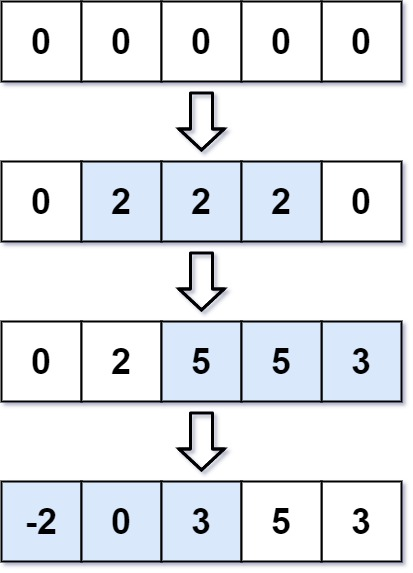
\includegraphics[width=0.2\linewidth]{images/lc0370_eg}
\label{fig:lc0370eg}
\end{figure}

\item Example 2
\begin{lstlisting}
length = 10, updates = [[2,4,6],[5,6,8],[1,9,-4]] --> [0,-4,2,2,2,4,4,-4,-4,-4]
\end{lstlisting}
\end{itemize}

\subsection*{Solution {\scriptsize\color{gray}\Coffeecup\hspace{1mm}Time $O(n)$, Space $O(1)$}}
\begin{lstlisting}
std::vector<int> getModifiedArray(int length, std::vector<std::vector<int>>& updates) {
  std::vector<int> arr(length, 0);
  for (const auto& update : updates) {
    int start_idx = update[0];
    int end_idx = update[1];
    int inc = update[2];
    arr[start_idx] += inc;
    if (end_idx + 1 < length) { arr[end_idx + 1] -= inc; }
  }
  for (int i = 1; i < length; ++i) { arr[i] += arr[i - 1]; }
  return arr;
}
\end{lstlisting}

\section{LC 0303 - Range Sum Query - Immutable}\label{lc0303}
\hyperref[sec:prefix_sum]{[Prefix Sum]}\\

Given a \ul{non-empty} integer array {\colorbox{CodeBackground}{\lstinline|nums|}}, handle multiple queries of the following type: \\

Calculate the sum of the elements of {\colorbox{CodeBackground}{\lstinline|nums|}} between indices {\colorbox{CodeBackground}{\lstinline|left|}} and {\colorbox{CodeBackground}{\lstinline|right|}} inclusive where {\colorbox{CodeBackground}{\lstinline|left <= right|}}.\\

Implement the {\colorbox{CodeBackground}{\lstinline|NumArray|}} class:
\begin{itemize}
\item {\colorbox{CodeBackground}{\lstinline|NumArray(int[] nums)|}} - Initializes the object with the integer array {\colorbox{CodeBackground}{\lstinline|nums|}}.
\item {\colorbox{CodeBackground}{\lstinline|int sumRange(int left, int right)|}} - Returns the sum of the elements of {\colorbox{CodeBackground}{\lstinline|nums|}} between indices {\colorbox{CodeBackground}{\lstinline|left|}} and {\colorbox{CodeBackground}{\lstinline|right|}} inclusive (i.e. {\colorbox{CodeBackground}{\lstinline|nums[left] + nums[left + 1] + ... + nums[right]|}}).
\end{itemize}

\subsection*{Solution 1 - Prefix Sum (size $n + 1$) {\scriptsize\color{gray}\Coffeecup\hspace{1mm}Time $O(n)$, Space $O(n)$}}
\begin{lstlisting}
class NumArray {
 public:
  NumArray(std::vector<int>& nums) {
    prefix_sum_.resize(nums.size() + 1, 0);
    for (int i = 0; i < nums.size(); ++i) { prefix_sum_[i + 1] = prefix_sum_[i] + nums[i]; }
  }

  int sumRange(int left, int right) { return prefix_sum_[right + 1] - prefix_sum_[left]; }

  std::vector<int> prefix_sum_;
};
\end{lstlisting}

\subsection*{Solution 2 - Prefix Sum (size $n$) {\scriptsize\color{gray}\Coffeecup\hspace{1mm}Time $O(n)$, Space $O(n)$}}
\begin{lstlisting}
class NumArray {
 public:
  NumArray(std::vector<int>& nums) {
    prefix_sum_.resize(nums.size(), 0);
    for (int i = 0; i < nums.size(); ++i) {
      prefix_sum_[i] = (i == 0 ? 0 : prefix_sum_[i - 1]) + nums[i];
    }
  }

  int sumRange(int left, int right) {
    return prefix_sum_[right] - (left == 0 ? 0 : prefix_sum_[left - 1]);
  }

 private:
  std::vector<int> prefix_sum_;
};
\end{lstlisting}

\subsection*{Related}
\begin{itemize}
\item \hyperref[lc0303]{LC 0303 - Range Sum Query - Immutable}
\item \hyperref[lc0304]{LC 0304 - Range Sum Query 2D - Immutable}
\end{itemize}

\section{LC 0238 - Product of Array Except Self}\label{lc0238}
\hyperref[sec:prefix_sum]{[Prefix Sum]}\\

Given an integer array {\colorbox{CodeBackground}{\lstinline|nums|}} ({\colorbox{CodeBackground}{\lstinline|nums.size() >= 2|}}), return an array {\colorbox{CodeBackground}{\lstinline|answer|}} such that {\colorbox{CodeBackground}{\lstinline|answer[i]|}} is equal to the product of all the elements of {\colorbox{CodeBackground}{\lstinline|nums|}} except {\colorbox{CodeBackground}{\lstinline|nums[i]|}}.\\

You must write an algorithm that runs in {\colorbox{CodeBackground}{\lstinline|O(n)|}} time and without using the division operation.\\

Examples:
\begin{itemize}
	\item {\colorbox{CodeBackground}{\lstinline|nums = [1,2,3,4] --> [24,12,8,6]|}}
	\item {\colorbox{CodeBackground}{\lstinline|nums = [-1,1,0,-3,3] --> [0,0,9,0,0]|}}
\end{itemize}

\subsection*{Solution 1 - Prefix \& Suffix Sum {\scriptsize\color{gray}\Coffeecup\hspace{1mm}Time $O(n)$, Space $O(n)$}}
\begin{lstlisting}
std::vector<int> productExceptSelf(std::vector<int>& nums) {
  int n = nums.size();
  std::vector<int> prefix_prod(n + 1, 1);
  for (int i = 0; i < n; ++i) { prefix_prod[i + 1] = prefix_prod[i] * nums[i]; }
  std::vector<int> suffix_prod(n + 1, 1);
  for (int i = n - 1; i >= 0; --i) { suffix_prod[i] = suffix_prod[i + 1] * nums[i]; }
  std::vector<int> res(n);
  for (int i = 0; i < n; ++i) { res[i] = prefix_prod[i] * suffix_prod[i + 1]; }
  return res;
}
\end{lstlisting}

\subsection*{Solution 1 - Prefix \& Suffix Sum, Optimized {\scriptsize\color{gray}\Coffeecup\hspace{1mm}Time $O(n)$, Space $O(n)$}}
\begin{lstlisting}
std::vector<int> productExceptSelf(std::vector<int>& nums) {
  int n = nums.size();
  std::vector<int> prefix_prod(n, 1);
  std::vector<int> suffix_prod(n, 1);
  for (int i = 1; i < n; ++i) { prefix_prod[i] = prefix_prod[i - 1] * nums[i - 1]; }
  for (int i = n - 2; i >= 0; --i) { suffix_prod[i] = suffix_prod[i + 1] * nums[i + 1]; }
  std::vector<int> res(n);
  for (int i = 0; i < n; ++i) { res[i] = prefix_prod[i] * suffix_prod[i]; }
  return res;
}
\end{lstlisting}

\section{LC 0560 - Subarray Sum Equals Target}\label{lc0560}
\hyperref[sec:prefix_sum]{[Prefix Sum]}\\

Given a \ul{non-empty} integer array {\colorbox{CodeBackground}{\lstinline|nums|}} and an integer {\colorbox{CodeBackground}{\lstinline|target|}}, return the number of subarrays whose sum equals to {\colorbox{CodeBackground}{\lstinline|target|}}.\\

Examples:
\begin{itemize}
\item {\colorbox{CodeBackground}{\lstinline|nums = [1,1,1], target = 2 --> 2|}}
\item {\colorbox{CodeBackground}{\lstinline|nums = [1,2,3], target = 3 --> 2|}}
\end{itemize}

\subsection*{*Solution 1 - Prefix Sum (Time Limit Exceeded) {\scriptsize\color{gray}\Coffeecup\hspace{1mm}Time $O(n^2)$, Space $O(n)$}}
\begin{lstlisting}
int subarraySum(std::vector<int>& nums, int target) {
  std::vector<int> prefix_sum(nums.size() + 1, 0);
  for (int i = 1; i <= nums.size(); ++i) { prefix_sum[i] = prefix_sum[i - 1] + nums[i - 1]; }
  int num_subarray = 0;
  for (int i = 0; i < nums.size(); ++i) {
    for (int j = i + 1; j <= nums.size(); ++j) {
      if (prefix_sum[j] - prefix_sum[i] == target) { ++num_subarray; }
    }
  }
  return num_subarray;
}

\end{lstlisting}

\subsection*{Solution 2 - Prefix Sum + Hash Map {\scriptsize\color{gray}\Coffeecup\hspace{1mm}Time $O(n)$, Space $O(n)$}}
\begin{lstlisting}
int subarraySum(std::vector<int>& nums, int target) {
  std::unordered_map<int, int> acc_sum2freq;
  int num_subarray = 0;
  int acc_sum = 0;
  acc_sum2freq[0] = 1;
  for (int num : nums) {
    acc_sum += num;
    if (acc_sum2freq.find(acc_sum - target) != acc_sum2freq.end()) {
      num_subarray += acc_sum2freq[acc_sum - target];
    }
    ++acc_sum2freq[acc_sum];
  }
  return num_subarray;
}
\end{lstlisting}

\subsection*{Related - Hash Map For Searching Two Related Elements}
\begin{itemize}
\item \hyperref[lc0001]{LC 0001 - Two Sum}
\item \hyperref[lc0560]{LC 0560 - Subarray Sum Equals Target}
\item \hyperref[lc0523]{LC 0523 - Subarray Sum is Multiple of Target}
\item \hyperref[lc0525]{LC 0525 - Binary Subarray with Equal Zeros and Ones}
\end{itemize}

\section{LC 0523 - Subarray Sum is Multiple of Target}\label{lc0523}
\hyperref[sec:prefix_sum]{[Prefix Sum]}\\

Given a \ul{non-empty} integer array {\colorbox{CodeBackground}{\lstinline|nums|}} ({\colorbox{CodeBackground}{\lstinline|nums[i] >= 0|}}) and an integer {\colorbox{CodeBackground}{\lstinline|target|}} ({\colorbox{CodeBackground}{\lstinline|target >= 1|}}), return {\colorbox{CodeBackground}{\lstinline|true|}} if {\colorbox{CodeBackground}{\lstinline|nums|}} has a \ul{good subarray} or {\colorbox{CodeBackground}{\lstinline|false|}} otherwise.\\

A \ul{good subarray} is a subarray where:
\begin{itemize}
\item its length is at least two, and
\item the sum of the elements of the subarray is a multiple of {\colorbox{CodeBackground}{\lstinline|target|}}.
\end{itemize}

Note that an integer {\colorbox{CodeBackground}{\lstinline|x|}} is a multiple of {\colorbox{CodeBackground}{\lstinline|target|}} if there exists an integer {\colorbox{CodeBackground}{\lstinline|n|}} such that {\colorbox{CodeBackground}{\lstinline|x = n * k|}}. {\colorbox{CodeBackground}{\lstinline|0|}} is always a multiple of {\colorbox{CodeBackground}{\lstinline|target|}}.\\

Examples:
\begin{itemize}
\item {\colorbox{CodeBackground}{\lstinline|nums = [23,2,4,6,7], target = 6 --> true ([2,4])|}}
\item {\colorbox{CodeBackground}{\lstinline|nums = [23,2,6,4,7], target = 6 --> true ([23,2,6,4,7])|}}
\item {\colorbox{CodeBackground}{\lstinline|nums = [23,2,6,4,7], target = 13 --> false|}}
\end{itemize}

\subsection*{*Solution 1 - Prefix Sum (Time Limit Exceeded) {\scriptsize\color{gray}\Coffeecup\hspace{1mm}Time $O(n^2)$, Space $O(n)$}}
\begin{lstlisting}
bool checkSubarraySum(std::vector<int>& nums, int target) {
  std::vector<int> prefix_sum(nums.size() + 1, 0);
  for (int i = 1; i <= nums.size(); ++i) { prefix_sum[i] = prefix_sum[i - 1] + nums[i - 1]; }
  for (int i = 0; i < nums.size() - 1; ++i) {
    for (int j = i + 2; j <= nums.size(); ++j) {
      if ((prefix_sum[j] - prefix_sum[i]) % target == 0) { return true; }
    }
  }
  return false;
}
\end{lstlisting}

\subsection*{Solution 2 - Prefix Sum + Hash Map {\scriptsize\color{gray}\Coffeecup\hspace{1mm}Time $O(n)$, Space $O(n)$}}
\begin{lstlisting}
bool checkSubarraySum(std::vector<int>& nums, int target) {
  std::unordered_map<int, int> acc_rem2idx;
  int acc_sum = 0;
  acc_rem2idx[0] = -1;
  for (int i = 0; i < nums.size(); ++i) {
    acc_sum += nums[i];
    int acc_rem = acc_sum % target;
    if (acc_rem2idx.find(acc_rem) != acc_rem2idx.end()) {
      if (i - acc_rem2idx[acc_rem] >= 2) { return true; }
    } else {  // store the earliest index for each remainder
      acc_rem2idx[acc_rem] = i;
    }
  }
  return false;
}
\end{lstlisting}

\subsection*{Related - Hash Map For Searching Two Related Elements}
\begin{itemize}
\item \hyperref[lc0001]{LC 0001 - Two Sum}
\item \hyperref[lc0560]{LC 0560 - Subarray Sum Equals Target}
\item \hyperref[lc0523]{LC 0523 - Subarray Sum is Multiple of Target}
\item \hyperref[lc0525]{LC 0525 - Binary Subarray with Equal Zeros and Ones}
\end{itemize}

\section{LC 0525 - Binary Subarray with Equal Zeros and Ones}\label{lc0525}
\hyperref[sec:prefix_sum]{[Prefix Sum]}\\

Given a \ul{non-empty} binary array {\colorbox{CodeBackground}{\lstinline|nums|}}, return the maximum length of a subarray with an equal number of {\colorbox{CodeBackground}{\lstinline|0|}} and {\colorbox{CodeBackground}{\lstinline|1|}}.\\

\begin{itemize}
\item {\colorbox{CodeBackground}{\lstinline|nums = [0,1] --> 2|}}
\item {\colorbox{CodeBackground}{\lstinline|nums = [0,1,0] --> 2|}}
\end{itemize}

\subsection*{Solution - Prefix Sum {\scriptsize\color{gray}\Coffeecup\hspace{1mm}Time $O(n)$, Space $O(n)$}}
\begin{lstlisting}
int findMaxLength(std::vector<int>& nums) {
  std::unordered_map<int, int> acc_sum2idx;
  int max_len = 0;
  int acc_sum = 0;
  acc_sum2idx[0] = -1;
  for (int i = 0; i < nums.size(); i++) {
    acc_sum += (nums[i] == 0) ? -1 : 1;
    if (acc_sum2idx.find(acc_sum) != acc_sum2idx.end()) {
      max_len = std::max(max_len, i - acc_sum2idx[acc_sum]);
    } else {  // store the earliest index for each acc_sum
      acc_sum2idx[acc_sum] = i;
    }
  }
  return max_len;
}
\end{lstlisting}

\subsection*{Related - Hash Map For Searching Two Related Elements}
\begin{itemize}
\item \hyperref[lc0001]{LC 0001 - Two Sum}
\item \hyperref[lc0560]{LC 0560 - Subarray Sum Equals Target}
\item \hyperref[lc0523]{LC 0523 - Subarray Sum is Multiple of Target}
\item \hyperref[lc0525]{LC 0525 - Binary Subarray with Equal Zeros and Ones}
\end{itemize}

\section{LC 0209 - Shortest Subarray Sum Greater or Equal to Target}\label{lc0209}
{\hyperref[sec:sliding_window]{[Sliding Window]}}

\begin{tcolorbox}
\begin{itemize}
\item Find the \ul{shortest subarray} whose sum is greater or equal to {\colorbox{CodeBackground}{\lstinline|target|}} in the given \ul{array}.
\end{itemize}
\end{tcolorbox}

Given a \ul{non-empty} array of integers {\colorbox{CodeBackground}{\lstinline|nums|}} ({\colorbox{CodeBackground}{\lstinline|nums[i] >= 1|}}) and a integer {\colorbox{CodeBackground}{\lstinline|target|}} ({\colorbox{CodeBackground}{\lstinline|target >= 1|}}), return the minimal length of a \ul{subarray} whose sum is greater than or equal to {\colorbox{CodeBackground}{\lstinline|target|}}. If there is no such subarray, return {\colorbox{CodeBackground}{\lstinline|0|}} instead.\\

Examples:
\begin{itemize}
\item {\colorbox{CodeBackground}{\lstinline|target = 7, nums = [2,3,1,2,4,3] --> 2 ([4,3])|}}
\item {\colorbox{CodeBackground}{\lstinline|target = 4, nums = [1,4,4] --> 1|}}
\item {\colorbox{CodeBackground}{\lstinline|target = 11, nums = [1,1,1,1,1,1,1,1] --> 0|}}
\end{itemize}

\subsection*{Solution - Sliding Window {\scriptsize\color{gray}\Coffeecup\hspace{1mm}Time $O(n)$, Space $O(1)$}}
\begin{lstlisting}
int minSubArrayLen(int target, std::vector<int>& nums) {
  int min_len = std::numeric_limits<int>::max();
  int sum = 0;
  int left = 0;
  for (int right = 0; right < nums.size(); ++right) {
    sum += nums[right];
    while (sum >= target) {
      min_len = std::min(min_len, right - left + 1);
      sum -= nums[left];
      ++left;
    }
  }
  return min_len == std::numeric_limits<int>::max() ? 0 : min_len;
}
\end{lstlisting}

\section{LC 1658 - Minimum Operations to Reduce X to Zero}\label{lc1658}
{\hyperref[sec:sliding_window]{[Sliding Window]}}

\begin{tcolorbox}
\begin{itemize}
\item Find the \ul{longest subarray} whose sum is equal to a target in the given \ul{array}.
\end{itemize}
\end{tcolorbox}

You are given a \ul{non-empty} integer array {\colorbox{CodeBackground}{\lstinline|nums|}} ({\colorbox{CodeBackground}{\lstinline|nums[i] >= 1|}}) and an integer {\colorbox{CodeBackground}{\lstinline|x|}} ({\colorbox{CodeBackground}{\lstinline|x >= 1|}}). \\

In one operation, you can either remove the \ul{leftmost} or the \ul{rightmost} element from {\colorbox{CodeBackground}{\lstinline|nums|}} and subtract its value from {\colorbox{CodeBackground}{\lstinline|x|}}. \\

Return the minimum number of operations to reduce {\colorbox{CodeBackground}{\lstinline|x|}} to \ul{exactly {\colorbox{CodeBackground}{\lstinline|0|}}} if it is possible, otherwise, return {\colorbox{CodeBackground}{\lstinline|-1|}}.\\

Examples:
\begin{itemize}
\item {\colorbox{CodeBackground}{\lstinline|nums = [1,1,4,2,3], x = 5 --> 2|}}
\item {\colorbox{CodeBackground}{\lstinline|nums = [5,6,7,8,9], x = 4 --> -1|}}
\item {\colorbox{CodeBackground}{\lstinline|nums = [3,2,20,1,1,3], x = 10 --> 5|}}
\end{itemize}

\subsection*{Solution - Sliding Window {\scriptsize\color{gray}\Coffeecup\hspace{1mm}Time $O(n)$, Space $O(1)$}}
\begin{lstlisting}
int minOperations(std::vector<int>& nums, int x) {
  int target = std::accumulate(nums.begin(), nums.end(), 0) - x;
  if (target < 0) { return -1; }
  int max_len = -1;
  int sum = 0;
  int left = 0;
  for (int right = 0; right < nums.size(); ++right) {
    sum += nums[right];
    while (sum > target) {
      sum -= nums[left];
      ++left;
    }
    if (sum == target) { max_len = std::max(max_len, right - left + 1); }
  }
  return max_len == -1 ? -1 : nums.size() - max_len;
}
\end{lstlisting}

\section{LC 1838 - Frequency of the Most Frequent Element after Increment}\label{lc1838}
{\hyperref[sec:sliding_window]{[Sliding Window]}}\\

You are given a \ul{non-empty} integer array {\colorbox{CodeBackground}{\lstinline|nums|}} ({\colorbox{CodeBackground}{\lstinline|nums[i] >= 1|}}) and an integer {\colorbox{CodeBackground}{\lstinline|k|}} ({\colorbox{CodeBackground}{\lstinline|k >= 1|}}). \\

In one operation, you can choose an index of {\colorbox{CodeBackground}{\lstinline|nums|}} and increment the element at that index by {\colorbox{CodeBackground}{\lstinline|1|}}.\\

Return the maximum possible frequency of an element after performing at most {\colorbox{CodeBackground}{\lstinline|k|}} operations.\\

Examples:
\begin{itemize}
\item {\colorbox{CodeBackground}{\lstinline|nums = [1,2,4], k = 5 --> 3 ([4,4,4])|}}
\item {\colorbox{CodeBackground}{\lstinline|nums = [1,4,8,13], k = 5 --> 2|}}\\
There are multiple optimal solutions:\\
- Increment the first element three times to make {\colorbox{CodeBackground}{\lstinline|nums = [4,4,8,13]|}}. \\
- Increment the second element four times to make {\colorbox{CodeBackground}{\lstinline|nums = [1,8,8,13]|}}. \\
- Increment the third element five times to make {\colorbox{CodeBackground}{\lstinline|nums = [1,4,13,13]|}}.
\item {\colorbox{CodeBackground}{\lstinline|nums = [3,9,6], k = 2 --> 1|}}
\end{itemize}

\subsection*{Solution - Sliding Window {\scriptsize\color{gray}\Coffeecup\hspace{1mm}Time $O(n)$, Space $O(1)$}}
We maintain a window in which the total number of operations required to equalize all elements does not surpass {\colorbox{CodeBackground}{\lstinline|k|}}.
\begin{lstlisting}
int maxFrequency(std::vector<int>& nums, int k) {
  std::sort(nums.begin(), nums.end());
  long num_op = 0;
  int max_freq = 1;
  int left = 0;
  for (int right = 1; right < nums.size(); ++right) {
    num_op += static_cast<long>(nums[right] - nums[right - 1]) * (right - left);
    while (num_op > k) {
      num_op -= nums[right] - nums[left];
      ++left;
    }
    max_freq = std::max(max_freq, right - left + 1);
  }
  return max_freq;
}
\end{lstlisting}

\section{LC 0239 - Sliding Window Maximum}\label{lc0239}
{\hyperref[sec:sliding_window]{[Sliding Window]}}\\

You are given a \ul{non-empty} array of integers {\colorbox{CodeBackground}{\lstinline|nums|}}, there is a sliding window of size {\colorbox{CodeBackground}{\lstinline|k|}} ({\colorbox{CodeBackground}{\lstinline|k >= 1|}}) which is moving from the very left of the array to the very right. You can only see the {\colorbox{CodeBackground}{\lstinline|k|}} numbers in the window. Each time the sliding window moves right by one position.\\

Return the list of max element for each window. \\

Examples:
\begin{itemize}
\item {\colorbox{CodeBackground}{\lstinline|nums = [1,3,-1,-3,5,3,6,7], k = 3 --> [3,3,5,5,6,7]|}}
\begin{lstlisting}
     Window Position           Max
--------------------------    -----
[1  3  -1] -3  5  3  6  7       3
 1 [3  -1  -3] 5  3  6  7       3
 1  3 [-1  -3  5] 3  6  7       5
 1  3  -1 [-3  5  3] 6  7       5
 1  3  -1  -3 [5  3  6] 7       6
 1  3  -1  -3  5 [3  6  7]      7
\end{lstlisting}
\item {\colorbox{CodeBackground}{\lstinline|nums = [1], k = 1 --> [1]|}}
\end{itemize}

\subsection*{Solution 1 - Brute Force}
\begin{lstlisting}
std::vector<int> maxSlidingWindow(std::vector<int>& nums, int k) {
  std::vector<int> max_elements;
  for (int i = 0; i < nums.size() - k + 1; ++i) {
    int maximum = std::numeric_limits<int>::min();
    for (int j = i; j < i + k; ++j) { maximum = std::max(maximum, nums[j]); }
    max_elements.push_back(maximum);
  }
  return max_elements;
}
\end{lstlisting}

\subsection*{Solution 2 - Deque}
\begin{lstlisting}
std::vector<int> maxSlidingWindow(std::vector<int>& nums, int k) {
  std::vector<int> max_elements;
  std::deque<int> window;
  for (int i = 0; i < nums.size(); ++i) {
    // Remove the indices that are out of the current window
    while (!window.empty() && window.front() <= i - k) { window.pop_front(); }

    // Remove indices from the back that are less than the current element
    while (!window.empty() && nums[i] >= nums[window.back()]) { window.pop_back(); }

    // Add the current index to the deque
    window.push_back(i);

    // If we've hit k elements, add the front of the deque to the result, as it's the max
    if (i >= k - 1) { max_elements.push_back(nums[window.front()]); }
  }

  return max_elements;
}
\end{lstlisting}

\section{LC 0480 - Sliding Window Median}\label{lc0480}
{\hyperref[sec:sliding_window]{[Sliding Window]}}\\

You are given a \ul{non-empty} integer array nums and an integer {\colorbox{CodeBackground}{\lstinline|k|}} ({\colorbox{CodeBackground}{\lstinline|k >= 1|}}). There is a sliding window of size {\colorbox{CodeBackground}{\lstinline|k|}} which is moving from the very left of the array to the very right. You can only see the {\colorbox{CodeBackground}{\lstinline|k|}} numbers in the window. Each time the sliding window moves right by one position.\\

Return the median array for each window in the original array. Answers within {\colorbox{CodeBackground}{\lstinline|10^-5|}} of the actual value will be accepted.\\

Examples:
\begin{itemize}
\item {\colorbox{CodeBackground}{\lstinline|nums = [1,3,-1,-3,5,3,6,7], k = 3 --> [1.00000,-1.00000,-1.00000,3.00000,5.00000,6.00000]|}}
\begin{lstlisting}
    Window Position            Median
--------------------------     -----
[1  3  -1] -3  5  3  6  7        1
 1 [3  -1  -3] 5  3  6  7       -1
 1  3 [-1  -3  5] 3  6  7       -1
 1  3  -1 [-3  5  3] 6  7        3
 1  3  -1  -3 [5  3  6] 7        5
 1  3  -1  -3  5 [3  6  7]       6
\end{lstlisting}
\item {\colorbox{CodeBackground}{\lstinline|nums = [1,2,3,4,2,3,1,4,2], k = 3 --> [2.00000,3.00000,3.00000,3.00000,2.00000,3.00000,2.00000]|}}
\end{itemize}

\section{LC 0274 - H-Index}
Given an array of integers {\colorbox{CodeBackground}{\lstinline|citations|}} where {\colorbox{CodeBackground}{\lstinline|citations[i]|}} is the number of citations a researcher received for their {\colorbox{CodeBackground}{\lstinline|i|}}th paper, return the researcher's \ul{h-index}.\\

The \ul{h-index} is defined as the maximum value of {\colorbox{CodeBackground}{\lstinline|h|}} such that the given researcher has published at least {\colorbox{CodeBackground}{\lstinline|h|}} papers that have each been cited at least {\colorbox{CodeBackground}{\lstinline|h|}} times.\\

Examples:
\begin{itemize}
	\item {\colorbox{CodeBackground}{\lstinline|citations = [3,0,6,1,5] --> 3|}}
	\item {\colorbox{CodeBackground}{\lstinline|citations = [1,3,1] --> 1|}}
\end{itemize}

\subsection*{Solution}
\begin{lstlisting}
int hIndex(std::vector<int>& citations) {
	std::sort(citations.begin(), citations.end(), std::greater<int>());
	int h_idx = 0;
	for (int i = 0; i < citations.size(); ++i) {
		if (citations[i] >= i + 1) {
			h_idx = i + 1;
		} else {
			break;
		}
	}
	return h_idx;
}
\end{lstlisting}

\section{LC 0042 - Trapping Rain Water}
Given {\colorbox{CodeBackground}{\lstinline|n|}} ({\colorbox{CodeBackground}{\lstinline|n >= 1|}}) non-negative integers representing an elevation map where the width of each bar is {\colorbox{CodeBackground}{\lstinline|1|}}, compute how much water it can trap after raining.\\

Example: {\colorbox{CodeBackground}{\lstinline|height = [0,1,0,2,1,0,1,3,2,1,2,1] --> 6|}}
\begin{figure}[H]
\centering
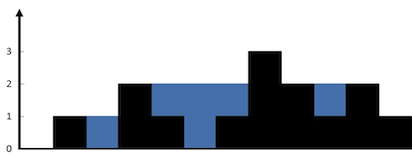
\includegraphics[width=0.4\linewidth]{images/lc0042_eg}
\end{figure}

\subsection*{Solution - Brute Force (Time Limit Exceeded)}\label{solution:lc0042_brute_force}
\begin{lstlisting}
int trap(std::vector<int>& heights) {
  int trapped_water = 0;
  for (int i = 1; i < heights.size() - 1; ++i) {
    int left_max_h = *std::max_element(heights.begin(), heights.begin() + i);
    int right_max_h = *std::max_element(heights.begin() + i + 1, heights.end());
    int height = std::min(left_max_h, right_max_h) - heights[i];
    trapped_water += height > 0 ? height : 0;
  }
  return trapped_water;
}
\end{lstlisting}

\subsection*{Solution - Brute Force, Optimized}\label{solution:lc0042_brute_force_optimized_1}
\begin{lstlisting}
int trap(std::vector<int>& heights) {
  if (heights.size() <= 2) { return 0; }
  int n = heights.size();
  std::vector<int> max_left_height(n, 0);
  std::vector<int> max_right_height(n, 0);
  max_left_height[0] = heights[0];
  for (int i = 1; i < n; ++i) {
    max_left_height[i] = std::max(heights[i], max_left_height[i - 1]);
  }
  max_right_height[n - 1] = heights[n - 1];
  for (int i = n - 2; i >= 0; --i) {
    max_right_height[i] = std::max(heights[i], max_right_height[i + 1]);
  }
  int trapped_water = 0;
  for (int i = 0; i < n; i++) {
    int height = std::min(max_left_height[i], max_right_height[i]) - heights[i];
    if (height > 0) { trapped_water += height; }
  }
  return trapped_water;
}
\end{lstlisting}

\subsection*{Solution - Brute Force, Optimized}\label{solution:lc0042_brute_force_optimized_2}
\begin{lstlisting}
int trap(std::vector<int>& heights) {
  int left_max_h = 0;
  int right_max_h = 0;
  int trapped_water = 0;
  int left = 0;
  int right = heights.size() - 1;
  while (left < right) {
    left_max_h = std::max(left_max_h, heights[left]);
    right_max_h = std::max(right_max_h, heights[right]);
    if (left_max_h < right_max_h) {
      trapped_water += left_max_h - heights[left];
      left++;
    } else {
      trapped_water += right_max_h - heights[right];
      right--;
    }
  }
  return trapped_water;
}
\end{lstlisting}

\subsection*{Other Solutions}
\begin{itemize}
%\item \hyperref[solution:lc0042_brute_force]{Brute Force (Time Limit Exceeded)}
%\item \hyperref[solution:lc0042_brute_force_optimized_1]{Brute Force, Optimized 1}
%\item \hyperref[solution:lc0042_brute_force_optimized_2]{Brute Force, Optimized 2}
\item \hyperref[solution:lc0042_monotonic_stack]{Monotonic Stack}
\end{itemize}
